\section{Постановка задачи}

\begin{frame}[shrink=15]{Актуальность}
    \footnotesize
    \begin{columns}[T,onlytextwidth]
        \begin{column}{0.48\textwidth}
            \begin{block}{Основные способы обучения роботов}
                \begin{itemize}
                    \item датасеты экспертных траекторий;
                    \item симуляторы с заданным подкрепляющим сигналом.
                \end{itemize}
            \end{block}
        \end{column}
        \begin{column}{0.48\textwidth}
            \begin{alertblock}{Проблемы переноса}
                \begin{itemize}
                    \item \textbf{Out-of-distribution:} реальные ситуации отсутствуют
                          в обучающем датасете;
                    \item \textbf{Sim-to-real:} симулятор не учитывает все особенности
                          реальной системы.
                \end{itemize}
            \end{alertblock}
        \end{column}
    \end{columns}

    \vspace{0.1em}
    \centering
    \normalsize
    Необходима адаптация робота (агента) непосредственно в реальной среде

    \vspace{0.3em}
    \begin{columns}[T,onlytextwidth]
        \begin{column}{0.55\textwidth}
            \begin{block}{Обучение с подкреплением}
                Агент обучается методом проб и ошибок непосредственно при
                взаимодействии со средой.

                \centering
                Исследование среды \(\rightarrow\) обнаружение эффективной
                последовательности действий \(\rightarrow\) достижение цели.
            \end{block}
        \end{column}
        \begin{column}{0.41\textwidth}
            \begin{alertblock}{Риски исследования}
                Случайное исследование в реальной среде может приводить к:
                \begin{itemize}
                    \item столкновениям;
                    \item поломке оборудования;
                    \item причинению вреда человеку.
                \end{itemize}
            \end{alertblock}
        \end{column}
    \end{columns}
    \vfill
    \begin{block}{Безопасное обучение с подкреплением (Safe RL)}
        Агент должен одновременно исследовать среду, достигать цели и соблюдать
        ограничения безопасности во время обучения и исполнения.
    \end{block}
\end{frame}

\begin{frame}{Цель и задачи исследования}
    \begin{block}{Цель работы}
        Исследование и разработка методов безопасного обучения с подкреплением,
        которые используют модели мира и иерархическую структуру поведения для
        повышения эффективности исследования среды при соблюдении ограничений
        безопасности в робототехнических задачах.
    \end{block}

    \small
    \textbf{Задачи исследования:}
    \begin{enumerate}
        \item Проанализировать методы безопасного обучения с подкреплением и
              среды для их экспериментальной оценки.
        \item Исследовать построение и агрегацию функций оценки будущих
              накопленных штрафов в модели мира.
        \item Разработать иерархический метод для уменьшения консервативности
              безопасной стратегии и улучшения исследования среды.
        \item Разработать метод генерации безопасных подцелей с использованием
              модели мира для задач с большим горизонтом.
        \item Разработать бенчмарк для обучения и оценки методов безопасного
              обучения с подкреплением в задачах с целями и ограничениями на
              естественном языке.
    \end{enumerate}
\end{frame}

\begin{frame}{Положения, выносимые на защиту}
    \small
    \begin{enumerate}
        \item Способ построения и агрегации функций оценки будущих накопленных
              штрафов в модели мира для безопасного исследования в рамках
              модели SPOWL.
        \item Метод SG-Safe, использующий генерацию промежуточных подцелей для
              улучшения исследовательских способностей безопасной стратегии.
        \item Метод ITES, контролирующий безопасность на уровне генерации
              подцелей и на уровне исполнения действий с помощью модели мира.
        \item Бенчмарк Caged CrafText для обучения и оценки методов обучения с
              подкреплением с естественно-языковыми целями и ограничениями.
    \end{enumerate}
\end{frame}

\begin{frame}[shrink=8]{Научная новизна}
    \footnotesize
    \begin{enumerate}
        \item В рамках метода \textbf{SPOWL} (Safe Planning and Policy Optimization
              via World Model Learning, безопасное планирование и оптимизация
              стратегии с использованием модели мира) предложена функция оценки
              будущих накопленных штрафов в рамках модели мира для улучшения
              скрытых представлений, а также для более точной оценки
              безопасности траекторий при планировании. Эксперименты на средах
              Safety Gym показали лучшую производительность и безопасность по
              сравнению с предыдущими методами безопасного обучения с
              подкреплением.
        \item Разработан метод \textbf{SG-Safe}, использующий промежуточные
              подцели для улучшения исследовательских способностей безопасной
              стратегии. Метод показывает лучшее качество в среде POLAMP в
              сравнении с методами безопасного обучения с подкреплением и
              методами на основе классического планирования.
        \item Разработан метод \textbf{ITES}, обеспечивающий безопасную генерацию
              и достижение подцелей с помощью модели мира. Метод достигает
              лучшего качества в задачах навигации и манипуляции с большим
              горизонтом в сравнении с методами на основе моделей мира в
              безопасном обучении с подкреплением.
        \item Разработан бенчмарк \textbf{Caged CrafText} для безопасного
              обучения с подкреплением с естественно-языковыми целями и
              ограничениями.
    \end{enumerate}

    \begin{block}{Соответствие паспорту специальности 1.2.1}
        \scriptsize
        \begin{itemize}
            \item постановка задач управления и принятия решений на основе
                  методов ИИ, в том числе управления роботами;
            \item разработка алгоритмического и программного обеспечения систем
                  ИИ, а также методов их взаимодействия с человеком;
            \item исследования доверенных систем ИИ: надёжность, устойчивость
                  и формирование тестовых наборов задач;
            \item методы и технологии поиска, приобретения и использования
                  знаний и закономерностей, в том числе эмпирических, в системах
                  искусственного интеллекта; исследования в области совместного
                  применения методов машинного обучения и классического
                  математического моделирования; методы и средства использования
                  экспертных знаний.
        \end{itemize}
    \end{block}
\end{frame}

\begin{frame}{Математическая постановка: CMDP}
    \begin{columns}[T,onlytextwidth]
        \begin{column}{0.53\textwidth}
            Марковский процесс принятия решений с ограничениями:
            \[
                \mathcal{M} =
                \langle \mathcal{S},\mathcal{A},P,r,c,\gamma,d \rangle ,
            \]
            где \(\mathcal{S}\) --- пространство состояний,
            \(\mathcal{A}\) --- пространство действий, \(P\) --- функция
            переходов, \(r\) --- вознаграждение, \(c\) --- штраф за нарушение
            ограничения, \(d\) --- допустимый бюджет нарушений.

            \[
                \max_{\pi}\;
                J_R(\pi)=
                \mathbb{E}_{\pi}\!\left[
                \sum_{t=0}^{\infty}\gamma^t r(s_t,a_t)\right]
            \]
            \[
                \text{при условии}\qquad
                J_C(\pi)=
                \mathbb{E}_{\pi}\!\left[
                \sum_{t=0}^{\infty}\gamma^t c(s_t,a_t)\right]\le d .
            \]
        \end{column}
        \begin{column}{0.43\textwidth}
            \begin{block}{Интерпретация}
                Стратегия должна максимизировать качество решения задачи,
                не превышая заданный уровень нарушений безопасности.
            \end{block}
            \begin{exampleblock}{Пример}
                Мобильный робот должен достигнуть цели, не сталкиваясь с
                препятствиями и не превышая допустимый уровень нарушений.
            \end{exampleblock}
        \end{column}
    \end{columns}
    \vfill
    {\scriptsize Источник постановки и сред: Altman, 1999; Ray et al.,
    ``Benchmarking Safe Exploration in Deep Reinforcement Learning'', 2019.}
\end{frame}

\begin{frame}[shrink=7]{Основные подходы к безопасному обучению с подкреплением}
    \begin{columns}[T,onlytextwidth]
        \begin{column}{0.49\textwidth}
            \begin{block}{Методы оптимизации стратегии с ограничениями}
                \textbf{Метод на основе функции Лагранжа}

                \[
                    \mathcal{L}(\pi,\lambda)
                    =
                    J_R(\pi)-\lambda\bigl(J_C(\pi)-d\bigr),
                    \qquad \lambda\geq 0 .
                \]
                \[
                    \max_{\pi}\min_{\lambda\geq 0}\mathcal{L}(\pi,\lambda).
                \]

                Если \(J_C(\pi)>d\), множитель \(\lambda\) увеличивается
                и стратегия сильнее штрафуется за нарушения.
            \end{block}

            \scriptsize
            \textbf{Плюс:} не требуется известная модель объекта управления.\\
            \textbf{Минус:} контролируется средний уровень нарушений, но не
            безопасность каждого действия.
        \end{column}

        \begin{column}{0.49\textwidth}
            \begin{block}{Методы на основе фильтрации действий}
                \textbf{Метод на основе барьерной функции}

                \(h\)~--- барьерная функция

                \(h(s)\geq 0\)~--- безопасное множество состояний

                \[
                    \nabla h(s)^\top\!\bigl(f(s)+g(s)a\bigr)
                    +\alpha\!\left(h(s)\right)\geq 0 .
                \]
                \[
                    a_{\mathrm{safe}}
                    =
                    \arg\min_a \|a-a_\pi\|^2 .
                \]
            \end{block}

            \scriptsize
            \textbf{Плюс:} может предотвращать небезопасные действия.\\
            \textbf{Минус:} обычно требует известной модели объекта управления,
            явного вида функции штрафов, их дифференцируемости и оптимизации на
            каждом шаге.
        \end{column}
    \end{columns}

    \vfill
    {\scriptsize Источники: Ray et al., 2019; Stooke et al., 2020; Ames et al., 2017; Dalal et al., 2018.}
\end{frame}

\begin{frame}[shrink=5]{Методы на основе модели мира}
    \begin{columns}[T,onlytextwidth]
        \begin{column}{0.52\textwidth}
            \begin{block}{Методы, использующие синтетический опыт и планирование}
                \textbf{SafeDreamer}

                \vspace{0.2em}
                использует латентную модель мира, которая предсказывает динамику
                скрытого состояния, вознаграждение и штрафы для планирования.
            \end{block}

            \vspace{0.3em}
            Модель мира обучается предсказывать: \(f_\theta\)~--- динамику среды,
            \(r_\theta\)~--- модель вознаграждений, \(c_\theta\)~--- модель штрафов:
            \[
                \begin{aligned}
                    \hat{s}_{t+1}&=f_\theta(\hat{s}_t,a_t),\\
                    \hat r_t&=r_\theta(\hat{s}_t,a_t),\qquad
                    \hat c_t=c_\theta(\hat{s}_t,a_t).
                \end{aligned}
            \]

            До выполнения действия агент оценивает кандидатные траектории:
            \[
                \max_{a_{0:H-1}}
                \sum_{t=0}^{H-1}\gamma^t\hat r_t
                \quad
                \text{при условии}\quad
                \sum_{t=0}^{H-1}\gamma^t\hat c_t\leq d.
            \]
        \end{column}
        \begin{column}{0.44\textwidth}
            \begin{block}{Преимущества}
                \begin{itemize}
                    \item оценка риска до взаимодействия с реальной средой;
                    \item планирование и обучение на воображаемых траекториях;
                    \item более эффективное использование опыта.
                \end{itemize}
            \end{block}

            \begin{alertblock}{Текущие проблемы}
                Проблема смещённой цели (\textit{miss objective}): декодер
                учится предсказывать ненужную информацию.

                \vspace{0.4em}
                Короткий горизонт планирования не учитывает штрафы, которые
                могут возникнуть после окончания кандидатной траектории.
            \end{alertblock}
        \end{column}
    \end{columns}
    \vfill
    {\scriptsize Источники: Huang et al., 2024; As et al., 2022; Jayant et al., 2022.}
\end{frame}

\section{SPOWL: оценка риска с помощью модели мира}

\begin{frame}{SPOWL: неявная модель мира}
    \footnotesize
    \begin{columns}[T,onlytextwidth]
        \begin{column}{0.50\textwidth}
            \centering
            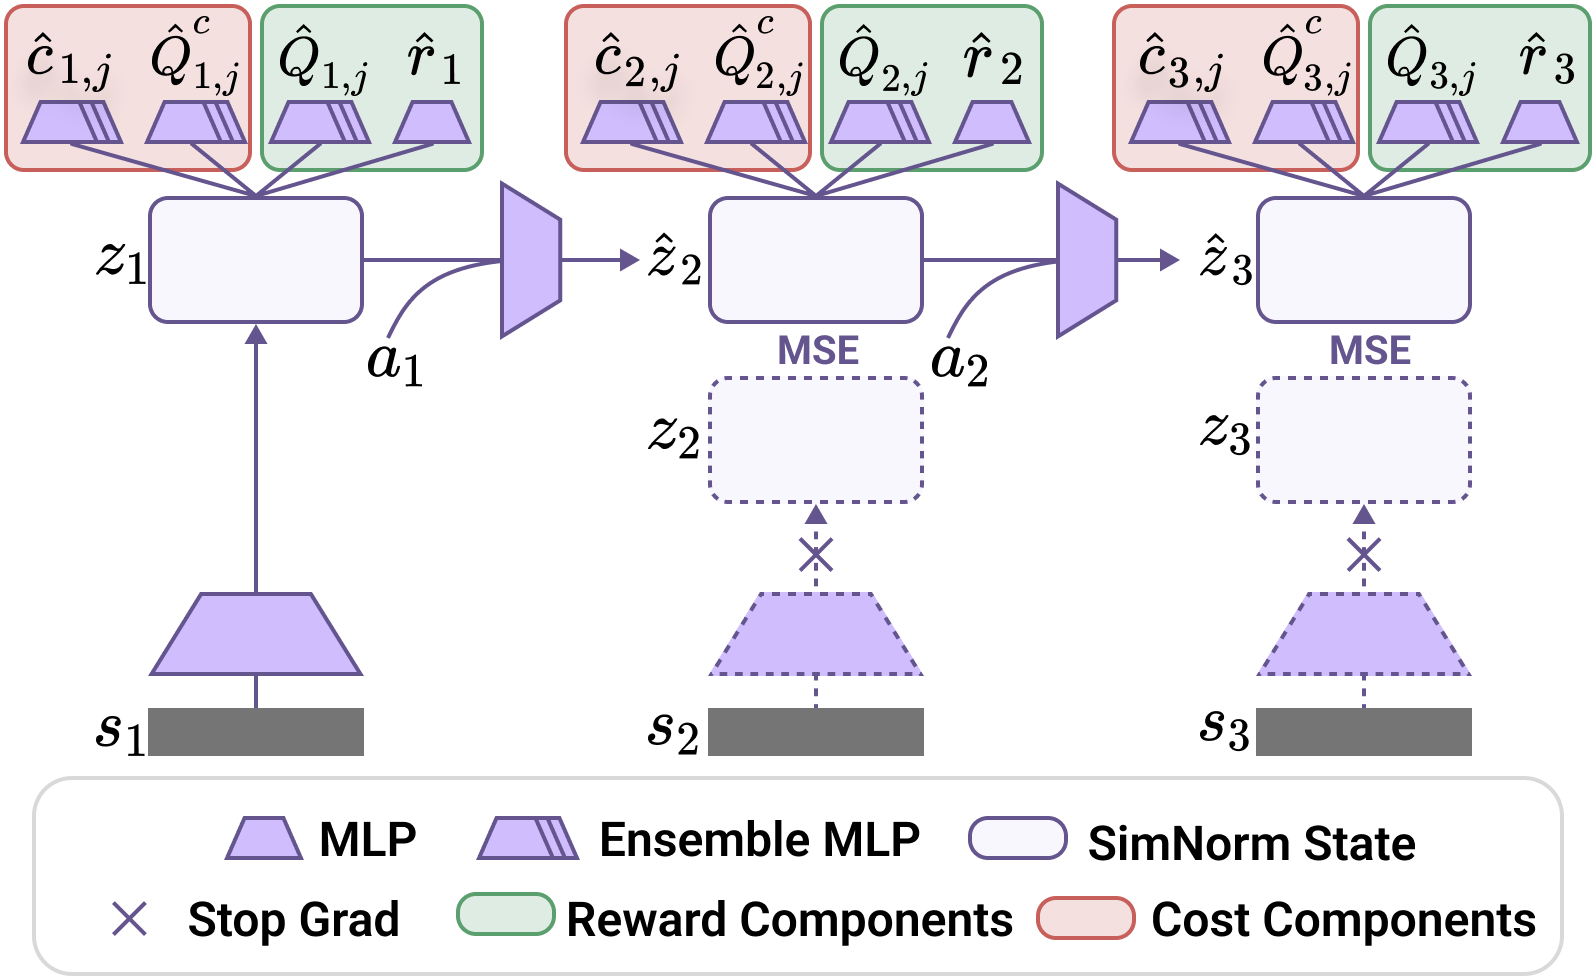
\includegraphics[width=\linewidth]{worldmodel}

            \vspace{0.2em}
            \scriptsize
            \[
                z_t=h(s_t), \qquad
                \hat z_{t+1}=f(z_t,a_t)
            \]
            \[
                \hat r_t=\hat R(z_t,a_t), \qquad
                \hat Q_{t,j}=\hat Q_j(z_t,a_t)
            \]
            \[
                \hat c_{t,j}=\hat C_j(z_t,a_t), \qquad
                \fcolorbox{red}{white}{\(\hat Q^c_{t,j}=\hat Q^c_j(z_t,a_t)\)}
            \]
            \vspace{0.1em}
            \hspace{0.50\linewidth}%
            {\scriptsize\textcolor{red}{%
                Дает информацию о будущих\\[0.05em]%
                \hspace{1.2em}штрафах%
            }}
        \end{column}
        \begin{column}{0.46\textwidth}
            \begin{block}{Неявная модель мира}
                Неявная модель мира в SPOWL обучается полезным представлениям
                с точки зрения CMDP-задачи и помогает решать проблему
                смещённой цели (\textit{miss objective}).
            \end{block}

            \begin{alertblock}{Оценка будущих накопленных штрафов}
                \[
                    Q_C(s,a)=
                    \mathbb{E}_{\pi}\!\left[
                    \sum_{k=0}^{\infty}\gamma^k c_{t+k}
                    \,\middle|\, s_t=s,\;a_t=a
                    \right].
                \]
            \end{alertblock}

            \scriptsize
            \(Q_C\) задаёт оценку ожидаемого будущего накопленного штрафа.
        \end{column}
    \end{columns}
\end{frame}

\begin{frame}[shrink=8]{SPOWL: оценка риска с помощью модели мира}
    \footnotesize
    \begin{columns}[T,onlytextwidth]
        \begin{column}{0.45\textwidth}
            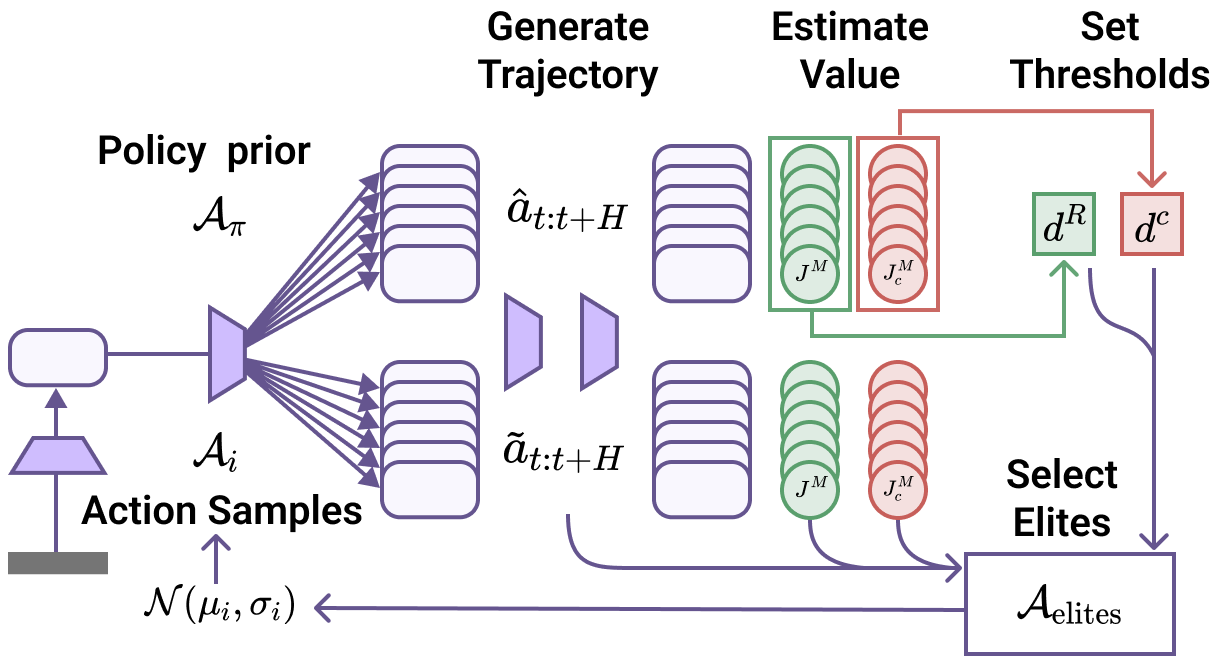
\includegraphics[width=\linewidth]{plan}
        \end{column}
        \begin{column}{0.51\textwidth}
            \begin{block}{Оценка кандидатной траектории}
                \[
                    \tau=(z_t,a_t,\ldots,z_{t+H},a_{t+H}),
                    \qquad
                    z_{t+1}=f(z_t,a_t)
                \]
                \[
                    a_t\sim\mathcal{N}(\mu_a,\sigma_a)
                    \quad \text{или} \quad
                    a_t\sim\pi(z_t).
                \]
            \end{block}

            \vspace{-0.3em}
            \[
                J_M=
                \sum_{i=0}^{H-1}\gamma^i\hat r_{t+i}
                +\gamma^H\hat Q_{\mathrm{avg}}(z_{t+H},a_{t+H})
            \]
            \[
                J_M^c=
                \sum_{i=0}^{H-1}\gamma_c^i\hat c_{\max,t+i}
                +\fcolorbox{red}{white}{\(\gamma_c^H
                \hat Q_{c,\mathrm{avg}}(z_{t+H},a_{t+H})\)}
            \]
            \vspace{-0.5em}
            \begin{center}
                \textcolor{red}{\scriptsize Улучшает оценку безопасности траекторий}
            \end{center}

            \vspace{0.2em}
            Это позволяет учитывать нарушения \textbf{за пределами короткого
            горизонта} модели мира.
        \end{column}
    \end{columns}
\end{frame}

\begin{frame}[shrink=12]{SPOWL: сравнение с базовыми методами}
    \setlength{\tabcolsep}{0.5pt}
    \renewcommand{\arraystretch}{0.68}
    \begin{columns}[T,onlytextwidth]
        \begin{column}{0.76\textwidth}
            \centering
            \tiny
    \resizebox{!}{0.50\textheight}{%
    \begin{tabular}{lr|rrrr}
        \toprule
        Task & Metric & \textbf{SPOWL} & TD-MPC2 & SafeDreamer & PPOLag(25) \\
        \midrule
        \multirow{3}{*}{PG1}
            & \(R\uparrow\) & \(26.9 \pm 0.4\) & \(27.5 \pm 0.2\) & \(12.0 \pm 4.0\) & \(14.5 \pm 0.6\) \\
            & \(C\downarrow\) & \(1.5 \pm 1.1\) & \(52.3 \pm 8.6\) & \(10.3 \pm 9.5\) & \(19.7 \pm 3.0\) \\
            & \(\rho\downarrow\) & \(133 \pm 2\) & \(515 \pm 9\) & \(160 \pm 16\) & \(361 \pm 20\) \\
        \midrule
        \multirow{3}{*}{PG2}
            & \(R\uparrow\) & \(13.7 \pm 3.2\) & \(27.4 \pm 0.5\) & \(5.2 \pm 3.9\) & \(2.0 \pm 0.9\) \\
            & \(C\downarrow\) & \(4.8 \pm 1.2\) & \(179.0 \pm 12.2\) & \(0 \pm 0\) & \(33.7 \pm 16.3\) \\
            & \(\rho\downarrow\) & \(280 \pm 5\) & \(1641 \pm 18\) & \(221 \pm 32\) & \(570 \pm 73\) \\
        \midrule
        \multirow{3}{*}{PP1}
            & \(R\uparrow\) & \(18.7 \pm 1.4\) & \(20.8 \pm 0.6\) & \(12.5 \pm 7.2\) & \(4.4 \pm 2.7\) \\
            & \(C\downarrow\) & \(1.8 \pm 2.5\) & \(34.2 \pm 11.6\) & \(7.3 \pm 10.4\) & \(24.2 \pm 12.4\) \\
            & \(\rho\downarrow\) & \(103 \pm 5\) & \(353 \pm 6\) & \(71 \pm 3\) & \(276 \pm 16\) \\
        \midrule
        \multirow{3}{*}{PB1}
            & \(R\uparrow\) & \(10.0 \pm 1.5\) & \(33.4 \pm 0.4\) & \(0.1 \pm 1.4\) & \(3.7 \pm 2.5\) \\
            & \(C\downarrow\) & \(5.4 \pm 2.7\) & \(103.3 \pm 3.1\) & \(0.3 \pm 0.5\) & \(33.6 \pm 7.7\) \\
            & \(\rho\downarrow\) & \(269 \pm 3\) & \(1219 \pm 10\) & \(159 \pm 3\) & \(392 \pm 27\) \\
        \midrule
        \multirow{3}{*}{CG1}
            & \(R\uparrow\) & \(31.3 \pm 0.8\) & \(34.8 \pm 0.3\) & \(6.6 \pm 1.2\) & \(18.4 \pm 3.9\) \\
            & \(C\downarrow\) & \(1.0 \pm 1.0\) & \(51.2 \pm 7.9\) & \(0 \pm 0\) & \(30.5 \pm 5.0\) \\
            & \(\rho\downarrow\) & \(113 \pm 2\) & \(563 \pm 11\) & \(127 \pm 15\) & \(345 \pm 9\) \\
        \midrule
        \multirow{3}{*}{DG1}
            & \(R\uparrow\) & \(19.0 \pm 1.9\) & \(27.9 \pm 1.5\) & \(1.1 \pm 0.9\) & \(0 \pm 0\) \\
            & \(C\downarrow\) & \(0.3 \pm 0.4\) & \(72.6 \pm 20.6\) & \(0 \pm 0\) & \(21.8 \pm 30.8\) \\
            & \(\rho\downarrow\) & \(286 \pm 15\) & \(659 \pm 33\) & \(260 \pm 70\) & \(376 \pm 70\) \\
        \midrule
        \multirow{3}{*}{AG1}
            & \(R\uparrow\) & \(38.9 \pm 1.4\) & \(61.0 \pm 2.6\) & \(0.2 \pm 0.2\) & \(5.1 \pm 3.9\) \\
            & \(C\downarrow\) & \(2.0 \pm 0.2\) & \(70.9 \pm 6.0\) & \(0 \pm 0\) & \(23.6 \pm 18.2\) \\
            & \(\rho\downarrow\) & \(275 \pm 6\) & \(682 \pm 6\) & \(218 \pm 58\) & \(638 \pm 115\) \\
        \bottomrule
    \end{tabular}}
        \end{column}
        \begin{column}{0.22\textwidth}
            \vspace{1.0em}
            \scriptsize
            \begin{block}{Метрики}
                \(R\uparrow\) --- среднее вознаграждение.

                \vspace{0.6em}
                \(C\downarrow\) --- средний штраф.

                \vspace{0.6em}
                \(\rho\downarrow\) --- средний штраф за шаг \((\times 10^4)\).
            \end{block}

            \vfill
            \centering
            \textbf{Safety Gym}\\[0.2em]
            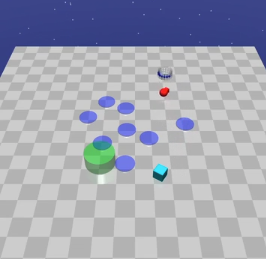
\includegraphics[width=0.9\linewidth]{safety_gym_point}
        \end{column}
    \end{columns}
\end{frame}

\begin{frame}{SPOWL: локальная и глобальная оценки штрафов}
    \centering
    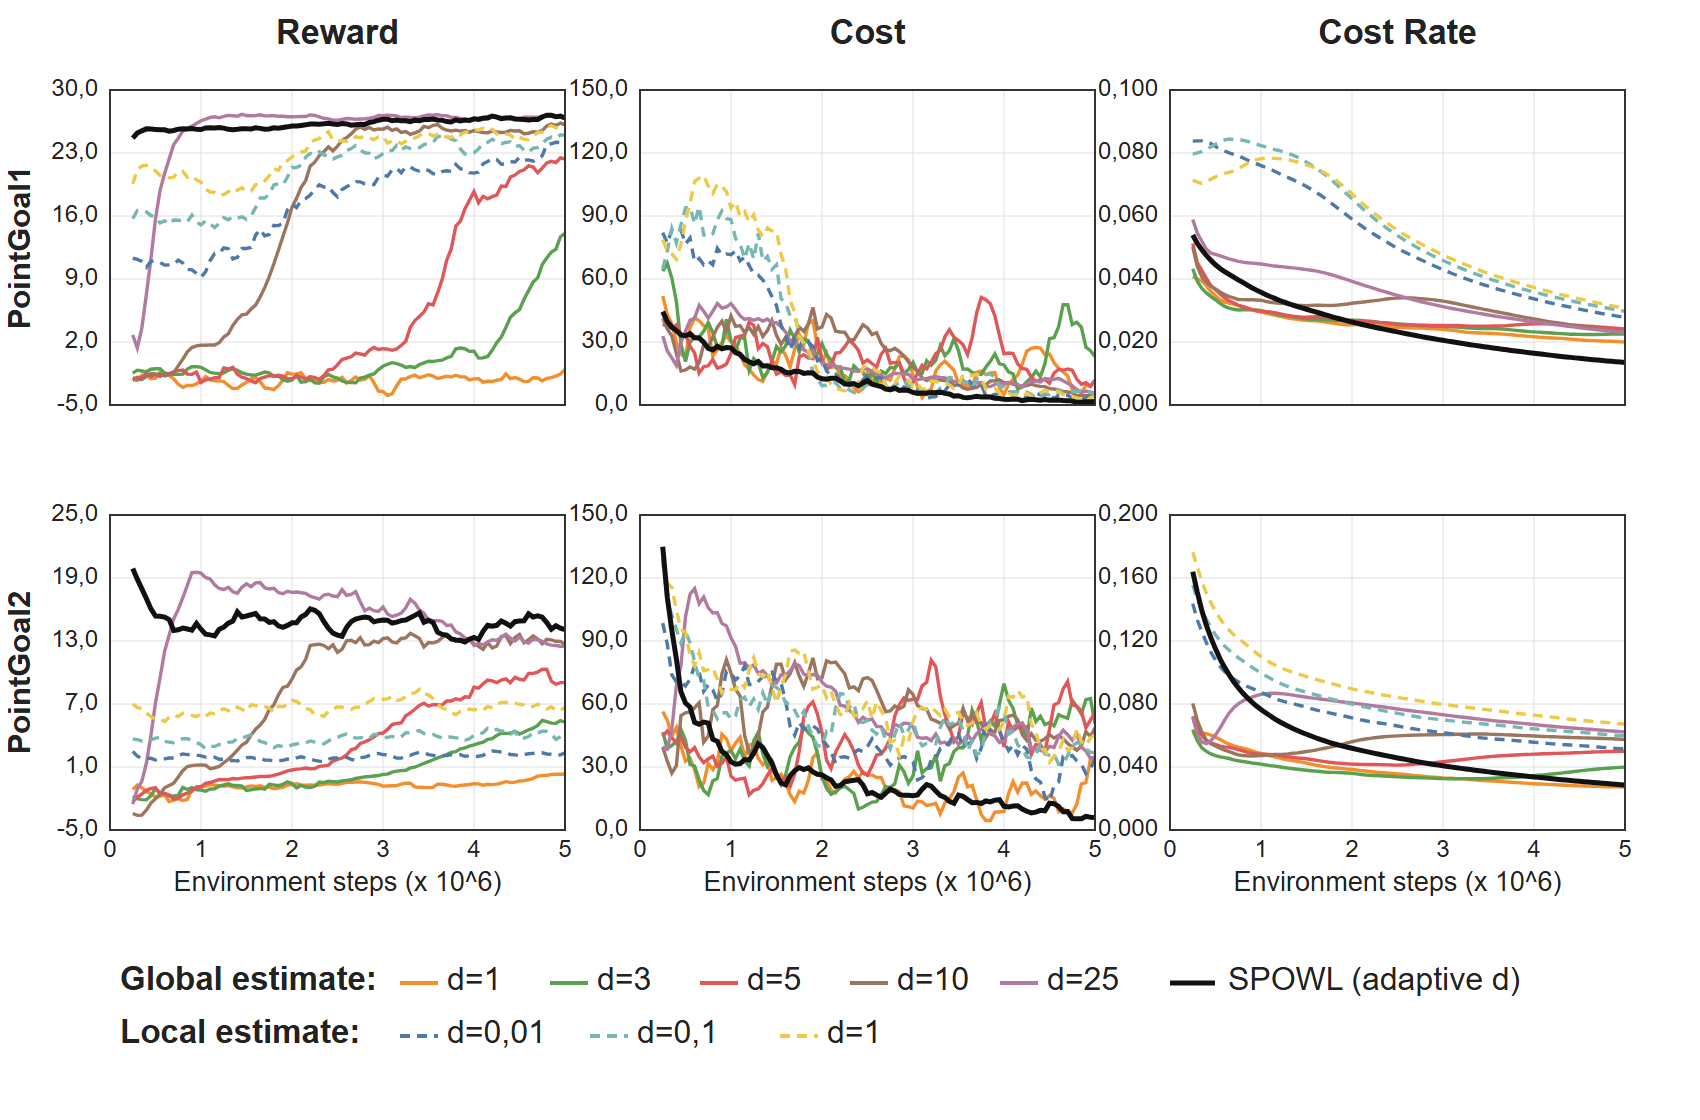
\includegraphics[height=0.76\textheight]{spowl_local_global_all_thresholds}
\end{frame}

\begin{frame}[shrink=8]{Проблема безопасного исследования в задачах с большим горизонтом}
    \begin{columns}[T,onlytextwidth]
        \begin{column}{0.43\textwidth}
            \begin{alertblock}{Почему задача сложна}
                В задачах с большим горизонтом агенту требуется найти
                длинную безопасную последовательность действий до получения
                полезного сигнала.
            \end{alertblock}

            \begin{itemize}
                \item большая последовательность шагов до цели;
                \item разреженное вознаграждение;
                \item большое пространство состояний и действий;
                \item ограничения безопасности могут преждевременно
                      подавлять исследование.
            \end{itemize}
        \end{column}

        \begin{column}{0.55\textwidth}
            \centering
            \scriptsize
            Базовые методы в задачах с большим горизонтом

            \vspace{0.25em}
            \textbf{SafeAntMaze-C}
            \vspace{0.1em}

            \tiny
            \setlength{\tabcolsep}{0.5pt}
            \renewcommand{\arraystretch}{0.72}
            \resizebox{0.74\linewidth}{!}{%
            \begin{tabular}{lcc}
                \toprule
                Method & Final SR$\uparrow$ & Final Cost$\downarrow$ \\
                \midrule
                SafeDreamer & \(0\) & \(13 \pm 18.11\) \\
                CUP & \(0\) & \(6.8 \pm 22.4\) \\
                FOCOPS & \(0\) & \(19.4 \pm 50.9\) \\
                TD3L/R & \(0.38 \pm 0.04\) & \(83.6 \pm 37.2\) \\
                PPOLAG & \(0.2 \pm 0.2\) & \(41.2 \pm 1.1\) \\
                TD3LAG & \(0.13 \pm 0.33\) & \(133.45 \pm 184.4\) \\
                \bottomrule
            \end{tabular}%
            }

            \vspace{0.45em}
            \textbf{SafePusher}
            \vspace{0.1em}

            \resizebox{0.74\linewidth}{!}{%
            \begin{tabular}{lcc}
                \toprule
                Method & Final SR$\uparrow$ & Final Cost$\downarrow$ \\
                \midrule
                SafeDreamer & \(0\) & \(6.7 \pm 2.7\) \\
                TD3LAG & \(0.05 \pm 0.03\) & \(54.72 \pm 3.16\) \\
                CUP & \(0.01\) & \(46.14 \pm 0.42\) \\
                FOCOPS & \(0\) & \(55.83 \pm 1.67\) \\
                PPOLAG & \(0\) & \(51.25 \pm 1.25\) \\
                \bottomrule
            \end{tabular}%
            }
        \end{column}
    \end{columns}
\end{frame}

\section{Безопасное исследование: SG-Safe}

\begin{frame}{SG-Safe: направленное исследование через подцели}
    \begin{columns}[T,onlytextwidth]
        \begin{column}{0.47\textwidth}
            \centering
            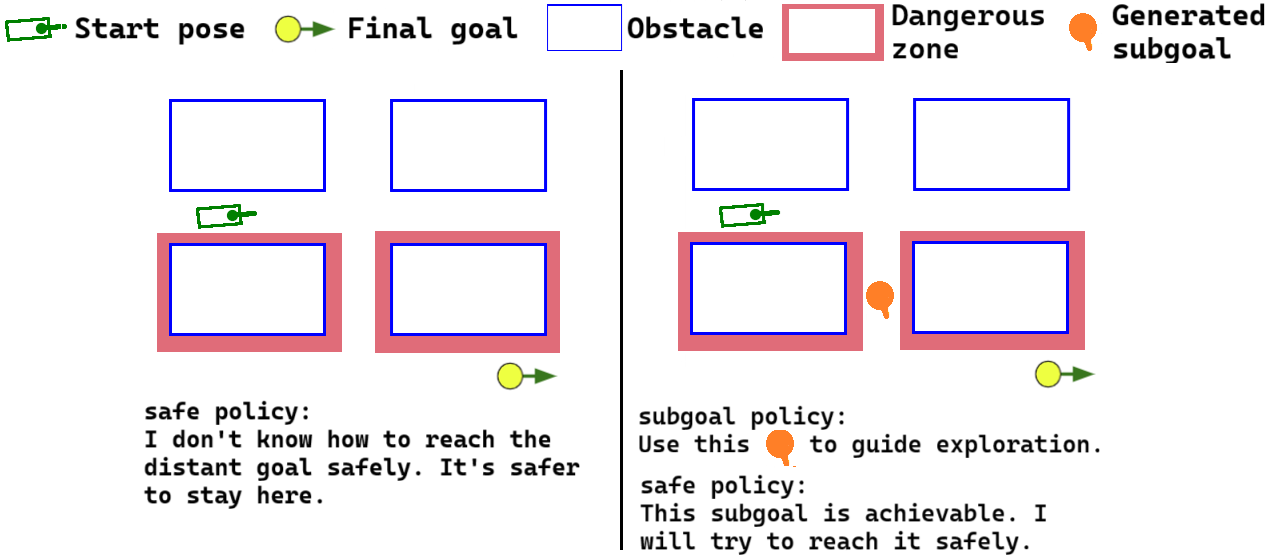
\includegraphics[width=\linewidth]{article_idea_env}

            \vspace{0.3em}
            \scriptsize
            Одноуровневая стратегия может не найти путь к удалённой цели;
            подцели направляют безопасное исследование.
        \end{column}
        \begin{column}{0.50\textwidth}
            \centering
            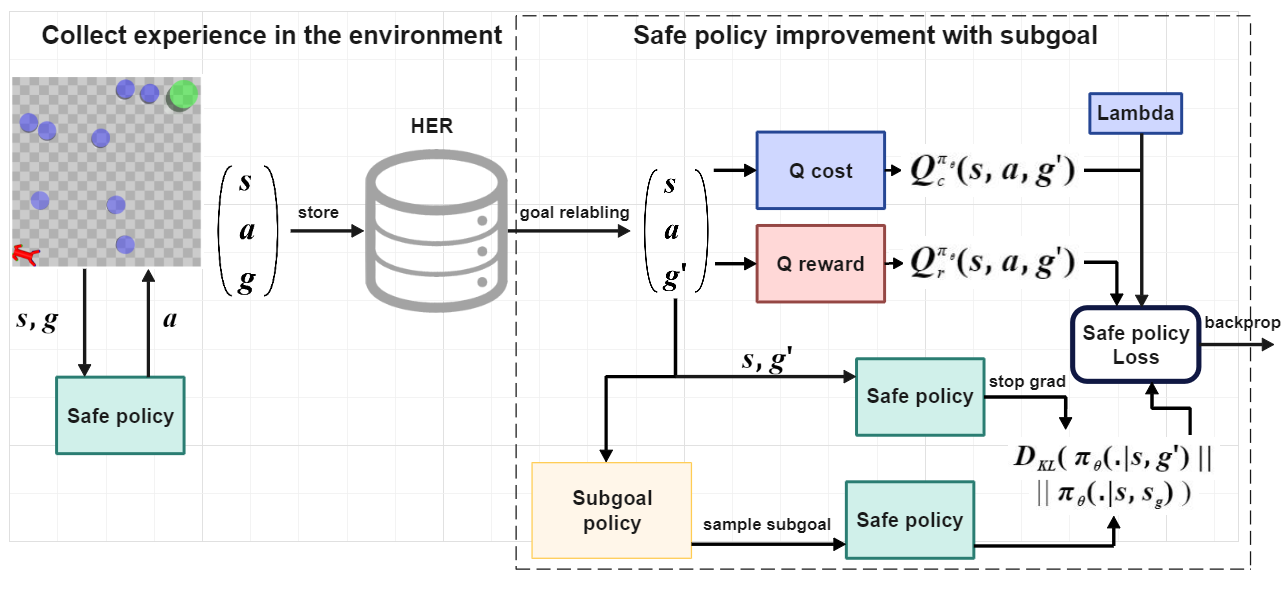
\includegraphics[width=\linewidth]{method_scheme_3}

            \vspace{0.3em}
            \scriptsize
            Промежуточные подцели декомпозируют задачу, направляют исследование
            и упрощают достижение цели; при обучении --- дополнительный сигнал,
            при исполнении --- только безопасная стратегия.
        \end{column}
    \end{columns}
\end{frame}

\begin{frame}[shrink=8]{SG-Safe: функции оптимизации стратегий}
    \scriptsize
    \begin{columns}[T,onlytextwidth]
        \begin{column}{0.49\textwidth}
            \textbf{Стратегия генерации подцелей}
            \[
                \pi^H =
                \arg\max_{\pi}
                \mathbb{E}\!\left[
                    A^{\pi^H_k}(s_g\mid s,g)
                \right],
            \]
            \[
                D_{\mathrm{KL}}\!\left(
                    \pi^H(\cdot\mid s,g)\,\|\,p_s(\cdot)
                \right)\leq\varepsilon .
            \]
            \[
                A^{\pi^H_k}(\hat s_g\mid s,g)
                =
                \mathbb{E}\!\left[
                    \psi_{\pi_\theta}(\hat s_g\mid s,g)
                    -
                    \psi_{\pi_\theta}(s_g\mid s,g)
                \right],
            \]
            \[
                \psi_{\pi_\theta}(s_g\mid s,g)
                =
                \max\!\left(
                    |V^{\pi_\theta}(s,s_g)|,\,
                    |V^{\pi_\theta}(s_g,g)|
                \right).
            \]

            Здесь \(V^{\pi_\theta}(s,g)\) --- ожидаемое дисконтированное
            вознаграждение при достижении цели \(g\) из состояния \(s\):
            \[
                V^{\pi_\theta}(s,g)
                =
                \mathbb{E}_{\pi_\theta}\!\left[
                    \sum_{t=0}^{\infty}\gamma^t
                    r(s_t,a_t,g)
                    \,\middle|\,s_0=s
                \right].
            \]
        \end{column}
        \begin{column}{0.49\textwidth}
            \textbf{Критики награды и штрафов}
            \[
                Q_r^{\pi_\theta}(s,a,g)
                =
                \mathbb{E}_{\pi_\theta}\!\left[
                    \sum_{t=0}^{\infty}\gamma^t r_t
                    \,\middle|\,s_0=s,a_0=a,g
                \right],
            \]
            \[
                Q_c^{\pi_\theta}(s,a,g)
                =
                \mathbb{E}_{\pi_\theta}\!\left[
                    \sum_{t=0}^{\infty}\gamma^t c_t
                    \,\middle|\,s_0=s,a_0=a,g
                \right].
            \]

            \textbf{Безопасная стратегия}
            \[
                \begin{aligned}
                J(\pi_\theta)=\mathbb{E}\big[&
                    Q_r^{\pi_\theta}(s,a,g)
                    -\lambda Q_c^{\pi_\theta}(s,a,g)\\[-0.2em]
                    &\fcolorbox{red}{white}{\(\displaystyle
                    -\alpha D_{\mathrm{KL}}\!\left(
                    \pi_\theta(\cdot\mid s,g)\,\|\,
                    \pi_\theta(\cdot\mid s,s_g)
                    \right)\)}\big].
                \end{aligned}
            \]
            \vspace{-0.8em}
            \begin{center}
                \scriptsize\textcolor{red}{Компонента для усиления исследования}
            \end{center}

            \begin{itemize}
                \item опыт переиспользуется с помощью HER;
                \item \(Q_r\) оценивает будущую награду, \(Q_c\) ---
                      будущие накопленные штрафы;
                \item выделенная KL-добавка направляет действия к подцели
                      и улучшает безопасное исследование.
            \end{itemize}
        \end{column}
    \end{columns}
\end{frame}

\begin{frame}[shrink=8]{SG-Safe: эксперименты на POLAMP}
    \centering
    \scriptsize
    SR~--- доля успешных эпизодов, CR~--- частота столкновений,
    MTSC~--- средний накопленный штраф за эпизод.
    Красным выделены методы с привилегированной информацией и/или
    явными моделями. Среднее~$\pm$~стандартное отклонение.

    \vspace{0.25em}
    \tiny
    \setlength{\tabcolsep}{2pt}
    \renewcommand{\arraystretch}{0.9}
    \begin{columns}[T,onlytextwidth]
        \begin{column}{0.49\textwidth}
            \centering
            \textbf{Level 1}
            \vspace{0.1em}

            \resizebox{\linewidth}{!}{%
            \begin{tabular}{lccc}
            \toprule
            Method & SR$\uparrow$ & CR$\downarrow$ & MTSC$\downarrow$ \\
            \midrule
            SG-Safe & $\mathbf{0.919\pm0.009}$ & $\mathbf{0.025\pm0.012}$ &
            $1.567\pm0.331$ \\
            SAC-LAG & $0.727\pm0.011$ & $0.029\pm0.009$ & $6.765\pm2.954$ \\
            SAC & $0.610\pm0.040$ & $0.023\pm0.014$ & $11.252\pm3.718$ \\
            SAC-NCMP & $0.427\pm0.000$ & $0.573\pm0.000$ &
            $\mathbf{0.869\pm0.015}$ \\
            \rowcolor{red!10} SAC-RCBF & $0.344\pm0.032$ & $0.240\pm0.025$ &
            $4.456\pm3.076$ \\
            ADVICE & $0.000\pm0.000$ & $0.031\pm0.000$ & $0.031\pm0.000$ \\
            \rowcolor{red!10} L-RRT & $0.551\pm0.152$ & $0.350\pm0.028$ &
            $8.335\pm1.898$ \\
            \bottomrule
            \end{tabular}%
            }
        \end{column}
        \begin{column}{0.49\textwidth}
            \centering
            \textbf{Level 2}
            \vspace{0.1em}

            \resizebox{\linewidth}{!}{%
            \begin{tabular}{lccc}
            \toprule
            Method & SR$\uparrow$ & CR$\downarrow$ & MTSC$\downarrow$ \\
            \midrule
            SG-Safe & $\mathbf{0.875\pm0.052}$ & $\mathbf{0.031\pm0.017}$ &
            $5.103\pm2.632$ \\
            SAC-LAG & $0.000\pm0.000$ & $\mathbf{0.004\pm0.006}$ &
            $1.319\pm0.802$ \\
            SAC & $0.000\pm0.000$ & $0.010\pm0.015$ & $5.054\pm2.325$ \\
            SAC-NCMP & $0.000\pm0.000$ & $1.000\pm0.000$ & $1.369\pm0.020$ \\
            \rowcolor{red!10} SAC-RCBF & $0.008\pm0.010$ & $0.050\pm0.025$ &
            $8.625\pm1.823$ \\
            ADVICE & $0.000\pm0.000$ & $0.010\pm0.000$ &
            $\mathbf{0.010\pm0.000}$ \\
            \rowcolor{red!10} L-RRT & $0.125\pm0.050$ & $0.664\pm0.165$ &
            $12.154\pm4.167$ \\
            \bottomrule
            \end{tabular}%
            }
        \end{column}
    \end{columns}

    \vspace{0.3em}
    \begin{columns}[T,onlytextwidth]
        \begin{column}{0.58\textwidth}
            \centering
            \textbf{Avg.}
            \vspace{0.1em}

            \resizebox{\linewidth}{!}{%
            \begin{tabular}{lccc}
            \toprule
            Method & SR$\uparrow$ & CR$\downarrow$ & MTSC$\downarrow$ \\
            \midrule
            SG-Safe & $\mathbf{0.897\pm0.026}$ & $0.028\pm0.010$ & $3.335\pm1.327$ \\
            SAC-LAG & $0.364\pm0.006$ & $\mathbf{0.017\pm0.005}$ & $4.042\pm1.530$ \\
            SAC & $0.305\pm0.020$ & $\mathbf{0.017\pm0.010}$ & $8.153\pm2.192$ \\
            SAC-NCMP & $0.214\pm0.000$ & $0.787\pm0.000$ & $1.119\pm0.012$ \\
            \rowcolor{red!10} SAC-RCBF & $0.176\pm0.017$ & $0.145\pm0.017$ &
            $6.541\pm1.788$ \\
            ADVICE & $0.000\pm0.000$ & $0.021\pm0.000$ & $\mathbf{0.021\pm0.000}$ \\
            \rowcolor{red!10} L-RRT & $0.338\pm0.080$ & $0.507\pm0.084$ &
            $10.245\pm2.289$ \\
            \bottomrule
            \end{tabular}%
            }
        \end{column}
        \begin{column}{0.38\textwidth}
            \vspace{0.9em}
            \centering
            \textbf{Среда POLAMP}\\
            \scriptsize навигационная задача с большим горизонтом
            \vspace{0.2em}

            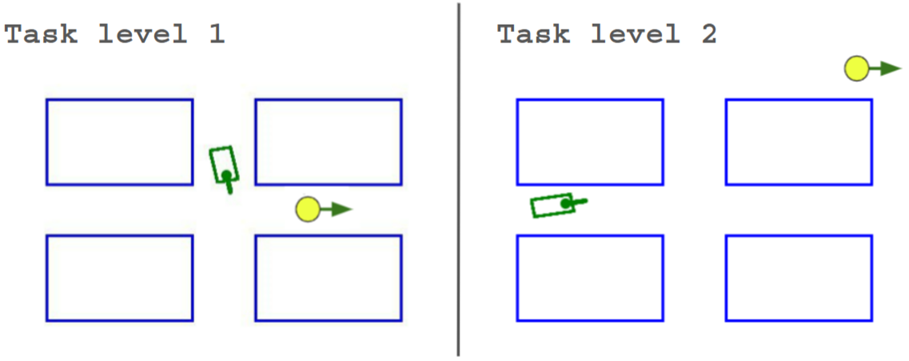
\includegraphics[width=\linewidth]{dataset_tasks_2}
        \end{column}
    \end{columns}
\end{frame}

\section{Безопасная иерархия: ITES}

\begin{frame}[shrink=5]{Развитие иерархического безопасного обучения с подкреплением с использованием модели мира}
    \begin{block}{Развитие иерархического безопасного обучения}
        \small
        В SG-Safe подцели направляют исследование, однако их безопасность явно
        не гарантируется. ITES решает более сильную задачу и контролирует
        безопасность всей иерархии: как при выборе промежуточных подцелей, так
        и при их достижении. Декомпозиция позволяет применять модель мира на
        коротком горизонте в задачах с длинной последовательностью действий.
    \end{block}
    \centering
    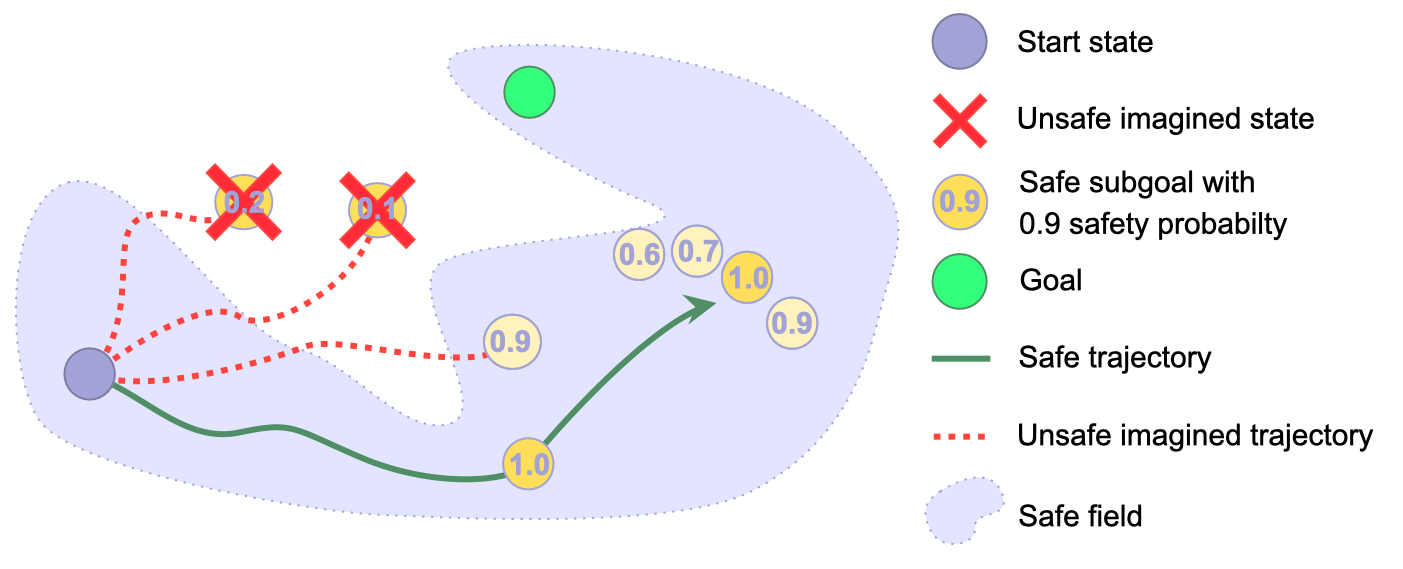
\includegraphics[height=0.56\textheight]{conceptual_scheme}
\end{frame}

\begin{frame}[shrink=10]{ITES: иерархическая структура и функции потерь}
    \begin{columns}[T,onlytextwidth]
        \begin{column}{0.44\textwidth}
            \begin{block}{Иерархия}
                \begin{itemize}
                    \item \(\pi^h_{\theta_h}(s_g\mid s,g)\) генерирует подцель;
                    \item \(\pi^l_{\theta_l}(a\mid s,s_g)\) достигает подцель.
                \end{itemize}
                {\small Верхнеуровневый критик вознаграждения}
                \[
                Q^h_{\theta_{qh}}(s,s_g,g)=
                \mathbb{E}\!\left[
                \sum_{t=0}^{T}\gamma^t r_t
                \,\middle|\,s_0=s,\ s_{g,0}=s_g,\ g
                \right].
                \]
                \vspace{0.2em}
                {\small Обучает эмбеддинги целей}
                \[
                \begin{aligned}
                L_{adj}=\mathbb{E}\big[&
                l\max(\|\psi(s_i)-\psi(s_j)\|-\epsilon,0)\\
                &+(1-l)\max(\epsilon+\delta\\
                &\quad-\|\psi(s_i)-\psi(s_j)\|,0)\big].
                \end{aligned}
                \]
            \end{block}
        \end{column}
        \begin{column}{0.53\textwidth}
            \begin{alertblock}{Функция потерь HRAC}
                \[
                L^h=-Q^h_{\theta_{qh}}(s,s_g,g)
                +\beta^h_{adj}L_{adj}(s,s_g).
                \]
            \end{alertblock}
            \small
            \(Q^h\) способствует максимизации вознаграждения от подцели для
            решения задачи.\\
            Член \(L_{adj}\) способствует генерации подцелей ровно на \(k\)
            шагов вперед.
        \end{column}
    \end{columns}
\end{frame}

\begin{frame}[shrink=8]{Безопасность на верхнем уровне: генерация безопасных подцелей}
    \begin{columns}[T,onlytextwidth]
        \begin{column}{0.47\textwidth}
            \begin{block}{Два сигнала безопасности}
                \small
                Модель штрафов возвращает вероятность того, что подцель
                принадлежит безопасному множеству:
                \[
                C_M(s_g,s)
                =\Pr(s_g\in\mathcal{S}_{safe}\mid s)\in[0,1].
                \]
                Верхнеуровневый критик штрафов оценивает ожидаемый
                дисконтированный накопленный штраф после выбора подцели:
                \[
                Q^h_c(s,s_g,g)=
                \mathbb{E}\!\left[
                \sum_{t=0}^{T}\gamma_c^t c_t
                \,\middle|\,s_0=s,\ s_{g,0}=s_g,\ g
                \right].
                \]
            \end{block}
        \end{column}
        \begin{column}{0.50\textwidth}
            \begin{alertblock}{Функция потерь ITES на верхнем уровне}
                \small
                \[
                \begin{aligned}
                L^h={}&-Q^h_{\theta_{qh}}(s,s_g,g)
                +\beta^h_{adj}L_{adj}(s,s_g)\\[0.3em]
                &+\fcolorbox{red}{white}{\(\displaystyle
                -\beta^h_{safe}C_M(s_g,s)
                +\lambda Q^h_c(s,s_g,g)\)}.
                \end{aligned}
                \]
                \centering
                \scriptsize\textcolor{red}{Компоненты, отвечающие за безопасность}
            \end{alertblock}
            \small
            \(C_M\) направляет подцель в безопасную область, а \(Q^h_c\)
            учитывает долгосрочные последствия её выбора.
        \end{column}
    \end{columns}
\end{frame}

\begin{frame}{Безопасность на нижнем уровне: безопасное достижение подцелей}
    \begin{columns}[T,onlytextwidth]
        \begin{column}{0.49\textwidth}
            \begin{alertblock}{Проблема}
                Даже безопасная подцель не гарантирует безопасную траекторию:
                агент может нарушить ограничения в процессе её достижения.
            \end{alertblock}
            \begin{block}{Проверка в модели мира}
                \small
                \begin{enumerate}
                    \item стратегия выбирает действие
                    \(a\sim\pi^l_{\theta_l}(a\mid s,s_g)\);
                    \item модель мира предсказывает
                    \(s'=M_{\theta_m}(s,a)\);
                    \item процедура повторяется для случайного горизонта
                    \(n\sim U(\{1,\ldots,k-1\})\).
                \end{enumerate}
            \end{block}
        \end{column}
        \begin{column}{0.48\textwidth}
            \begin{alertblock}{Функция потерь ITES на нижнем уровне}
                \small
                \[
                \begin{aligned}
                L^l={}&-Q^l_{\theta_{ql}}(s,a,s_g)\\
                &+\fcolorbox{red}{white}{\(\displaystyle
                -\beta^l_{safe}C_M(\phi(s_n),s)\)}.
                \end{aligned}
                \]
                \centering
                \scriptsize\textcolor{red}{Компонент, отвечающий за безопасность}
            \end{alertblock}
            \small
            \(C_M\) оценивает безопасность траектории в модели мира.
        \end{column}
    \end{columns}
\end{frame}

\begin{frame}[shrink=8]{Задачи навигации и манипуляции с большим горизонтом}
    \centering
    \scriptsize
    Итоговые результаты на SafeAntMaze и SafePusher.
    SAM-C~--- SafeAntMaze C-shape, SAM-W~--- SafeAntMaze W-shape,
    SR~--- доля успешных эпизодов.
    Методы с Final Cost~$\leqslant d$ выделены зелёным, нарушающие~---
    красным. Усреднение по 5 запускам.

    \vspace{0.2em}
    \tiny
    \setlength{\tabcolsep}{1pt}
    \renewcommand{\arraystretch}{0.75}
    \begin{columns}[T,onlytextwidth]
        \begin{column}{0.49\textwidth}
            \centering
            \textbf{SAM-C}
            \vspace{0.1em}

            \resizebox{0.82\linewidth}{!}{%
            \begin{tabular}{lcc}
            \toprule
            Method & Final SR$\uparrow$ & Final Cost$\downarrow$ \\
            \midrule
            \rowcolor{green!10} ITES & $\mathbf{0.88 \pm 0.01}$ & $15.2 \pm 17.3$ \\
            \rowcolor{green!10} SafeDreamer & $0$ & $13 \pm 18.11$ \\
            \rowcolor{green!10} CUP & $0$ & $\mathbf{6.8 \pm 22.4}$ \\
            \rowcolor{green!10} FOCOPS & $0$ & $19.4 \pm 50.9$ \\
            \rowcolor{red!10} TD3L/R & $0.38 \pm 0.04$ & $83.6 \pm 37.2$ \\
            \rowcolor{red!10} PPOLAG & $0.2 \pm 0.2$ & $41.2 \pm 1.1$ \\
            \rowcolor{red!10} TD3LAG & $0.13 \pm 0.33$ & $133.45 \pm 184.4$ \\
            \bottomrule
            \end{tabular}%
            }
        \end{column}
        \begin{column}{0.49\textwidth}
            \centering
            \textbf{SAM-W}
            \vspace{0.1em}

            \resizebox{0.82\linewidth}{!}{%
            \begin{tabular}{lcc}
            \toprule
            Method & Final SR$\uparrow$ & Final Cost$\downarrow$ \\
            \midrule
            \rowcolor{green!10} ITES & $\mathbf{0.35 \pm 0.05}$ & $183 \pm 16.5$ \\
            \rowcolor{green!10} TD3L/R & $0.05 \pm 0.02$ & $154 \pm 13.5$ \\
            \rowcolor{green!10} CUP & $0$ & $\mathbf{103.5 \pm 21.5}$ \\
            \rowcolor{green!10} FOCOPS & $0$ & $141.0 \pm 26.0$ \\
            \rowcolor{green!10} TD3LAG & $0$ & $128.68 \pm 210$ \\
            \rowcolor{green!10} PPOLAG & $0$ & $105 \pm 20.1$ \\
            \rowcolor{red!10} SafeDreamer & $0$ & $216.3 \pm 199$ \\
            \bottomrule
            \end{tabular}%
            }
        \end{column}
    \end{columns}

    \vspace{0.25em}
    \textbf{Pusher}
    \vspace{0.1em}

    \resizebox{0.42\linewidth}{!}{%
    \begin{tabular}{lcc}
    \toprule
    Method & Final SR$\uparrow$ & Final Cost$\downarrow$ \\
    \midrule
    \rowcolor{green!10} ITES & $\mathbf{0.42 \pm 0.02}$ & $\mathbf{12.8 \pm 0.87}$ \\
    \rowcolor{green!10} SafeDreamer & $0$ & $6.7 \pm 2.7$ \\
    \rowcolor{red!10} TD3LAG & $0.05 \pm 0.03$ & $54.72 \pm 3.16$ \\
    \rowcolor{red!10} CUP & $0.01$ & $46.14 \pm 0.42$ \\
    \rowcolor{red!10} FOCOPS & $0$ & $55.83 \pm 1.67$ \\
    \rowcolor{red!10} PPOLAG & $0$ & $51.25 \pm 1.25$ \\
    \bottomrule
    \end{tabular}%
    }
\end{frame}

\begin{frame}{ITES: абляция компонентов безопасности}
    \centering
    \begin{columns}[T,onlytextwidth]
        \begin{column}{0.49\textwidth}
            \centering
            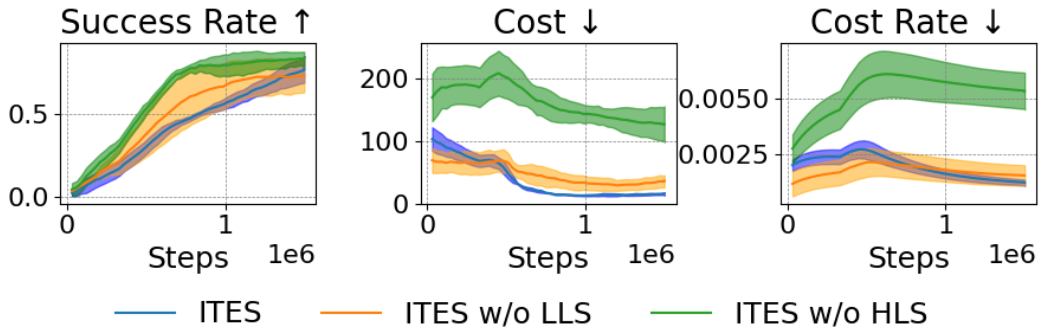
\includegraphics[width=\linewidth]{Ablation_SafeAntMazeCshape_3}
        \end{column}
        \begin{column}{0.49\textwidth}
            \centering
            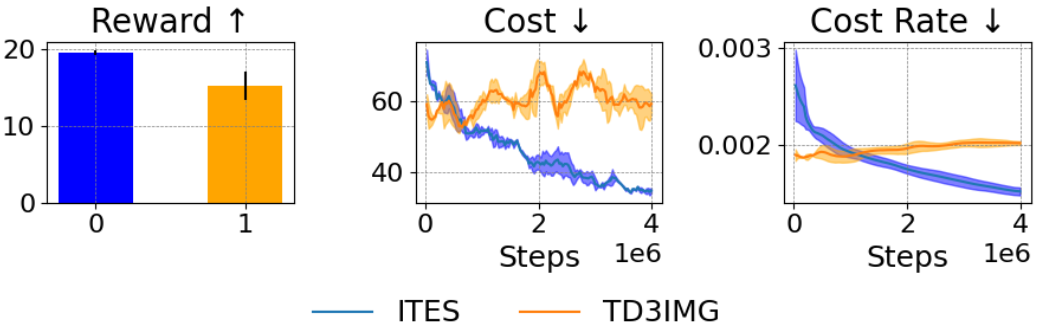
\includegraphics[width=\linewidth]{Ablation_PointGoal1_2}
        \end{column}
    \end{columns}

    \vspace{0.2em}
    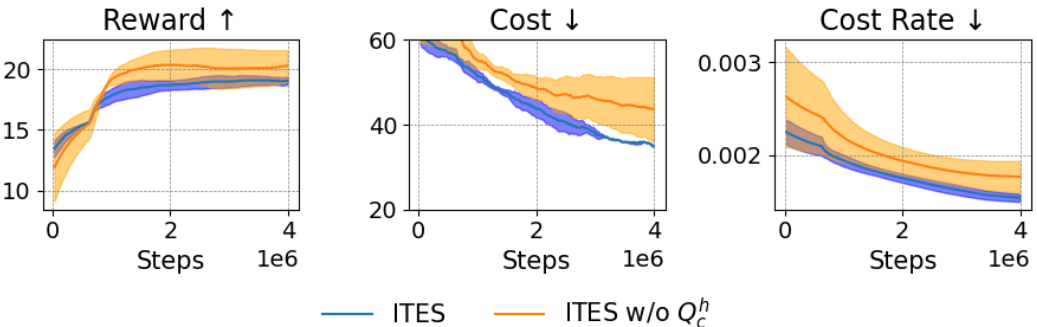
\includegraphics[width=0.55\linewidth]{Ablation_PointGoal1_Q_cost}

    \vspace{0.15em}
    \parbox{0.96\linewidth}{\scriptsize
    \textbf{Слева}: анализ безопасности на нижнем и верхнем уровнях
    (ITES w/o LLS и ITES w/o HLS на SafeAntMazeCshape).
    \textbf{Справа}: сравнение ITES без верхнеуровневой стратегии и
    полного ITES на PointGoal1.
    \textbf{Снизу}: сравнение ITES и ITES без верхнеуровневого
    критика штрафов \(Q^h_c\) на PointGoal1.
    Усреднение по 5 запускам.}
\end{frame}

\section{Текстовые ограничения: Caged CrafText}

\begin{frame}{Мультимодальная безопасность с языковыми целями и ограничениями}
    \begin{columns}[T,onlytextwidth]
        \begin{column}{0.52\textwidth}
            \begin{block}{Переход к естественному языку}
                \small
                В предыдущих главах цель и ограничения задавались формально:
                координатой цели или численной функцией штрафов.
            \end{block}
            \small
            В реальных сценариях пользователь формулирует на естественном языке
            не только цель, но и ограничения: каких объектов избегать, какие
            ресурсы сохранять и какие действия допустимы только при выполнении
            условий.

            \vspace{0.4em}
            Поэтому агент должен одновременно понимать текст, соотносить его
            с наблюдениями среды и принимать безопасные решения.
        \end{column}
        \begin{column}{0.45\textwidth}
            \centering
            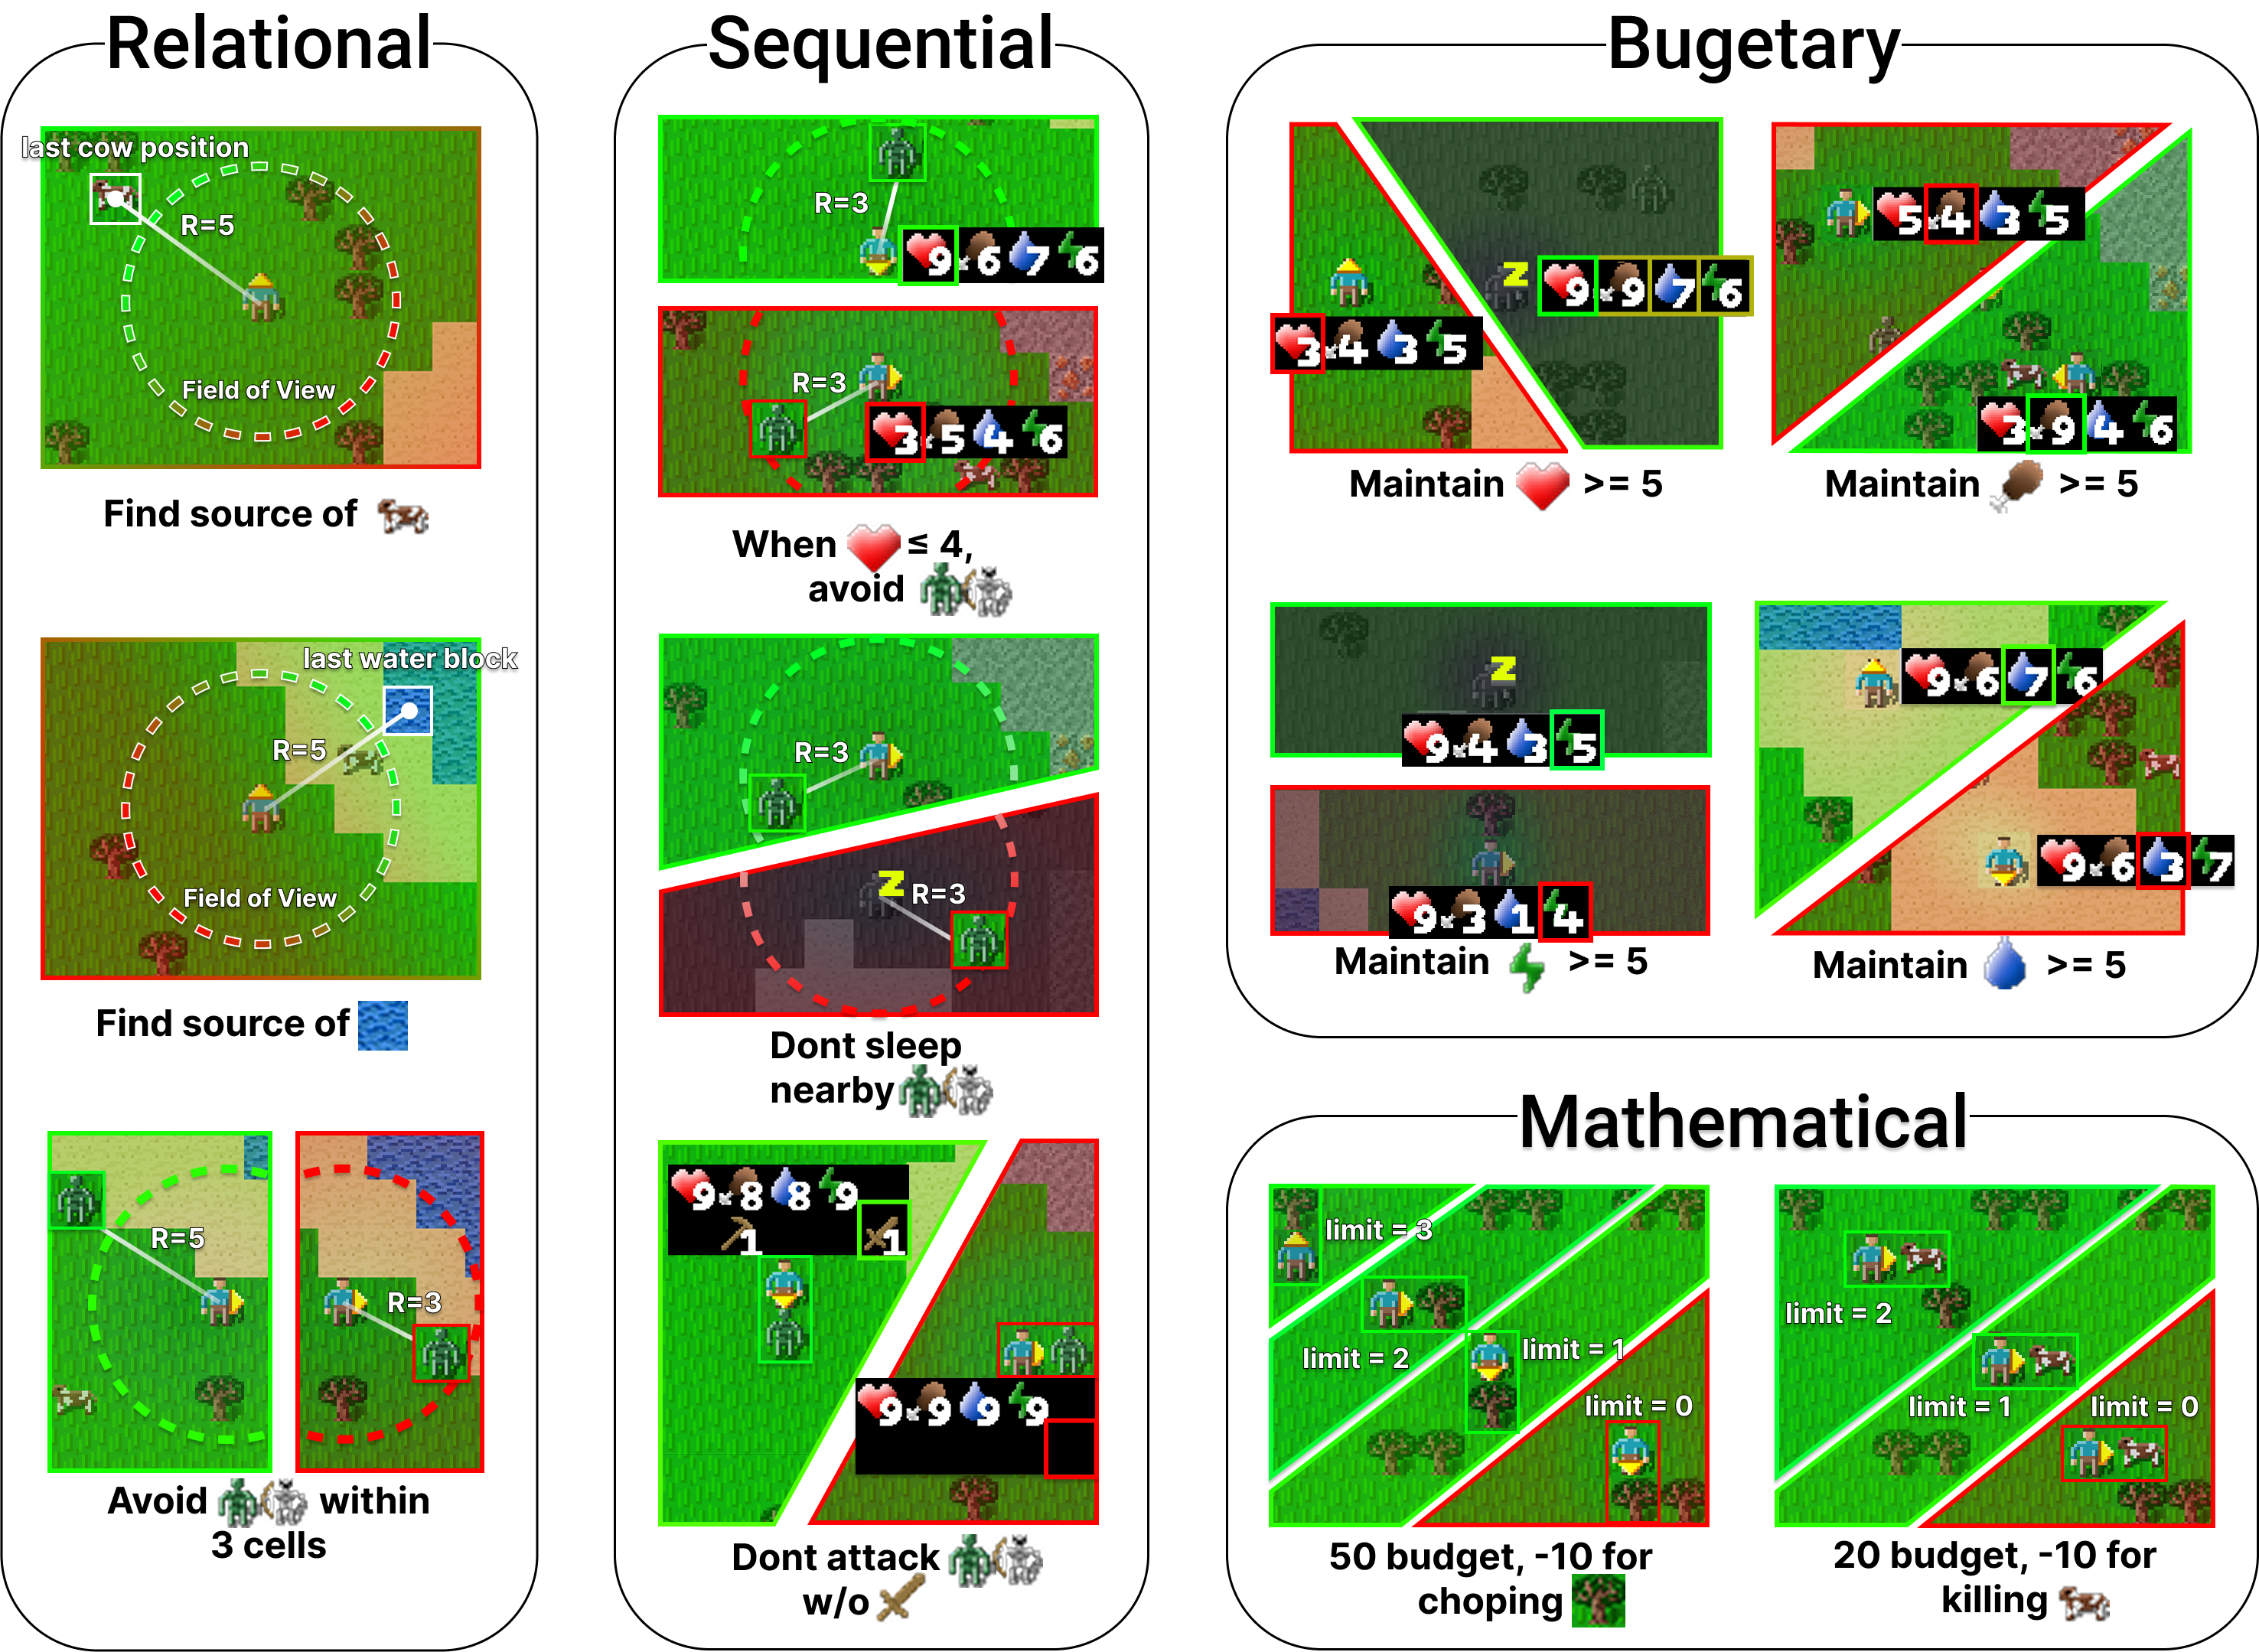
\includegraphics[width=\linewidth]{visual_abstract_3}
            \vspace{0.2em}

            \scriptsize Caged CrafText: цели и ограничения задаются естественным языком.
        \end{column}
    \end{columns}
\end{frame}

\newcommand{\cemj}[1]{\raisebox{-0.18ex}{\includegraphics[height=1.15em]{emoji/#1}}}

\begin{frame}{Caged CrafText: цели и ограничения на естественном языке}
    \begin{columns}[T,onlytextwidth]
        \begin{column}{0.75\textwidth}
            \small
            \textbf{Таблица 12. Таксономия задач Caged CrafText}

            \vspace{0.25em}
            \scriptsize
            \setlength{\tabcolsep}{3pt}
            \renewcommand{\arraystretch}{1.0}
            \begin{tabular}{@{}p{0.17\linewidth}p{0.48\linewidth}ccccc@{}}
                \hline
                \textbf{Сценарий} & \textbf{Ограничение} &
                \textbf{M} & \textbf{DE} & \textbf{SE} & \textbf{R} & \textbf{LU} \\
                \hline
                Budgetary & Maintain \cemj{food.png} \(\geq 5\) & \checkmark & \checkmark & \checkmark & & \\
                & Maintain \cemj{drink.png} \(\geq 5\) & \checkmark & \checkmark & \checkmark & & \\
                & Maintain \cemj{energy.png} \(\geq 5\) & & & \checkmark & & \\
                & Maintain \cemj{health.png} \(\geq 5\) & \checkmark & \checkmark & \checkmark & \checkmark & \\
                \hline
                Sequential & Don't attack \cemj{zombie.png}\cemj{skeleton.png} w/o \cemj{wood_sword.png} & & \checkmark & \checkmark & \checkmark & \\
                & Don't sleep nearby \cemj{zombie.png}\cemj{skeleton.png} & & & \checkmark & \checkmark & \\
                & When \cemj{health.png} \(\leq 4\), avoid \cemj{zombie.png}\cemj{skeleton.png} & & & \checkmark & \checkmark & \\
                \hline
                Mathematical & 20 budget, \(-10\) for killing \cemj{cow.png} & \checkmark & & \checkmark & \checkmark & \\
                & 50 budget, \(-10\) for chopping \cemj{tree.png} & \checkmark & & \checkmark & \checkmark & \\
                \hline
                Relational & Avoid \cemj{zombie.png}\cemj{skeleton.png} within 3 cells & \checkmark & & \checkmark & \checkmark & \\
                & Find source of \cemj{drink.png} & \checkmark & \checkmark & \checkmark & & \\
                & Find source of \cemj{food.png} & \checkmark & \checkmark & \checkmark & & \\
                \hline
                \textbf{Budgetary All} & & \checkmark & \checkmark & \checkmark & \checkmark & \\
                \textbf{Sequential All} & & & \checkmark & \checkmark & \checkmark & \\
                \textbf{Mathematical All} & & \checkmark & & \checkmark & \checkmark & \\
                \textbf{Relational All} & & \checkmark & \checkmark & \checkmark & \checkmark & \\
                \hline
                \textbf{Caged} & & \checkmark & \checkmark & \checkmark & \checkmark & \checkmark \\
                \hline
            \end{tabular}

            \vspace{0.15em}
            \scriptsize
            M~--- память, DE~--- глубокое исследование, SE~--- безопасное
            исследование, R~--- рассуждение, LU~--- понимание языка.
        \end{column}
        \begin{column}{0.23\textwidth}
            \scriptsize
            \centering
            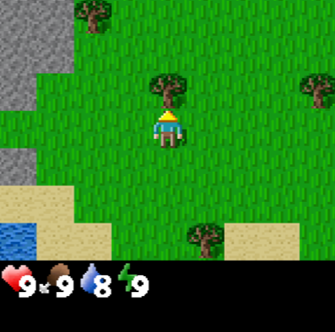
\includegraphics[width=\linewidth,height=0.36\textheight,keepaspectratio]{craftext_env}

            \vspace{0.8em}
            \begin{block}{Четыре типа ограничений}
                \begin{itemize}
                    \item бюджетные;
                    \item последовательные;
                    \item математические;
                    \item отношенческие.
                \end{itemize}
            \end{block}
        \end{column}
    \end{columns}
\end{frame}

\begin{frame}{Caged CrafText: сравнение базовых методов}
    \begin{columns}[c,onlytextwidth]
        \begin{column}{0.59\textwidth}
            \vfill
            \centering
            \scriptsize
            \(R\uparrow\) --- эпизодическое вознаграждение,
            \(C\downarrow\) --- эпизодический штраф.

            \vspace{0.35em}
            \tiny
            \setlength{\tabcolsep}{3pt}
            \setlength{\extrarowheight}{2pt}
            \renewcommand{\arraystretch}{1.25}
            \resizebox{\linewidth}{!}{%
            \begin{tabular}{lrrrrrrrr}
                \hline
                \multirow{2}{*}{\textbf{Набор задач}} &
                \multicolumn{2}{c}{\textbf{PPO}} &
                \multicolumn{2}{c}{\textbf{PPO-LAG}} &
                \multicolumn{2}{c}{\textbf{PPO-Cost}} &
                \multicolumn{2}{c}{\textbf{LLM}} \\
                & \(R\uparrow\) & \(C\downarrow\) & \(R\uparrow\) & \(C\downarrow\) &
                \(R\uparrow\) & \(C\downarrow\) & \(R\uparrow\) & \(C\downarrow\) \\
                \hline
                Budgetary All \((d=0.1)\) & 0.23 & 11.38 & 0.05 & 0.36 & 0.11 & \textbf{0.12} & 0.19 & 40.1 \\
                Sequential All \((d=0.1)\) & \textbf{0.24} & 7.65 & 0.05 & 1.02 & 0.08 & \textbf{0.82} & 0.19 & 22.7 \\
                Mathematical All \((d=0.1)\) & 0.23 & 110.42 & \textbf{0.24} & 0.10 & 0.18 & \textbf{0.05} & 0.19 & 16.9 \\
                Relational All \((d=10)\) & \textbf{0.22} & 31.36 & 0.11 & 11.69 & 0.04 & \textbf{8.18} & 0.18 & 15.2 \\
                \hline
                \textbf{Caged} \((d=0.1)\) & \textbf{0.22} & 103.66 & 0.03 & 0.17 & 0.14 & \textbf{0.13} & 0.20 & 43.4 \\
                \hline
            \end{tabular}}

            \vspace{0.35em}
            \scriptsize
            Результаты усреднены по 5 случайным сидам.
            \vfill
        \end{column}

        \begin{column}{0.39\textwidth}
            \centering
            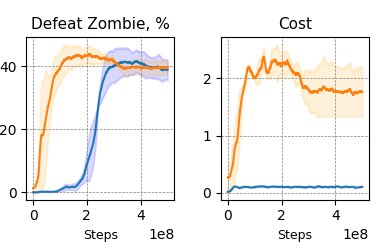
\includegraphics[width=0.88\linewidth,keepaspectratio]{Ablation_defeat_zombie_only}

            \scriptsize
            Ограничение: Don't attack w/o \(\cemj{wood_sword.png}\).

            \vspace{0.15em}
            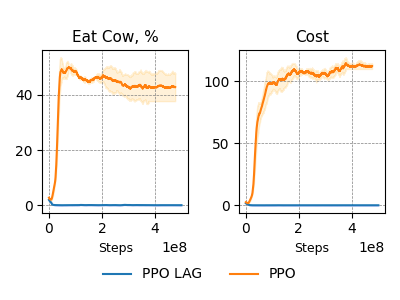
\includegraphics[width=0.88\linewidth,keepaspectratio]{Ablation_math_eat_cow}

            \scriptsize
            Ограничение: \(20\) budget, \(-10\) for killing \(\cemj{cow.png}\).

            \vspace{0.2em}
            \scriptsize
            \textcolor{blue}{\rule{1.3em}{0.35ex}}~PPO-LAG
            \quad
            \textcolor{orange}{\rule{1.3em}{0.35ex}}~PPO
        \end{column}
    \end{columns}
\end{frame}

\section{Итоги работы}

\begin{frame}{Практическая значимость}
    \begin{itemize}
        \item Компоненты SPOWL для оценки будущих накопленных штрафов
              применимы в робототехнических задачах безопасного исследования:
              агент заранее оценивает риск кандидатных действий до их выполнения
              в реальной среде.
        \item SG-Safe и ITES применимы к адаптации мобильных роботов в задачах
              автономной инспекции, патрулирования, обследования аварийных зон,
              навигации в шахтах и других труднодоступных пространствах.
        \item Репозитории с открытым кодом: SPOWL\footnote{\url{https://github.com/AIRI-Institute/SPOWL}}, SG-Safe\footnote{\url{https://github.com/Gricha1/SPEIS}}, ITES\footnote{\url{https://github.com/Gricha1/ITES_alg}}, CrafText\footnote{\url{https://github.com/AIRI-Institute/CrafText}}, Caged CrafText\footnote{\url{https://github.com/Gricha1/CAGED-CrafText}}.
    \end{itemize}
\end{frame}

\begin{frame}[shrink=5]{Публикации и апробация по теме диссертационной работы}
    \footnotesize
    \begin{columns}[T,onlytextwidth]
        \begin{column}{0.50\textwidth}
            \textbf{Публикации по теме работы:}

            \vspace{0.2em}
            Основные результаты по теме диссертации изложены в 5 публикациях:
            2~--- в журналах категории~К1 собственного перечня журналов МФТИ,
            2~--- в сборниках трудов конференций уровня~A и~A*,
            1~--- в виде препринта на arXiv.

            \vspace{0.25em}
            \begin{itemize}
                \item \textbf{SG-Safe}~--- журнал Technologies издательства MDPI, 2026,
                      категория~К1 перечня МФТИ, Q1;
                \item \textbf{Caged CrafText}~--- журнал Optical Memory and Neural
                      Networks, 2026, категория~К1;
                \item \textbf{SPOWL}~--- материалы ECAI 2025, конференция
                      уровня~A;
                \item \textbf{CrafText benchmark}~--- ACL 2025,
                      конференция уровня~A*;
                \item \textbf{ITES}~--- препринт arXiv:2606.22509, 2026.
            \end{itemize}
        \end{column}
        \begin{column}{0.46\textwidth}
            \textbf{Апробация результатов:}

            \vspace{0.2em}
            Основные результаты диссертационной работы докладывались
            и обсуждались на:

            \vspace{0.25em}
            \begin{itemize}
                \item международной конференции European Conference on
                      Artificial Intelligence, ECAI 2025 (метод SPOWL);
                \item конференции Fall into ML 2025;
                \item междисциплинарной конференции по искусственному
                      интеллекту «ИИ-АЗАМАН 2025»;
                \item семинарах Центра когнитивного моделирования МФТИ
                      (2023--2025).
            \end{itemize}
        \end{column}
    \end{columns}
\end{frame}
